\begin{figure}[h] 
\centering 
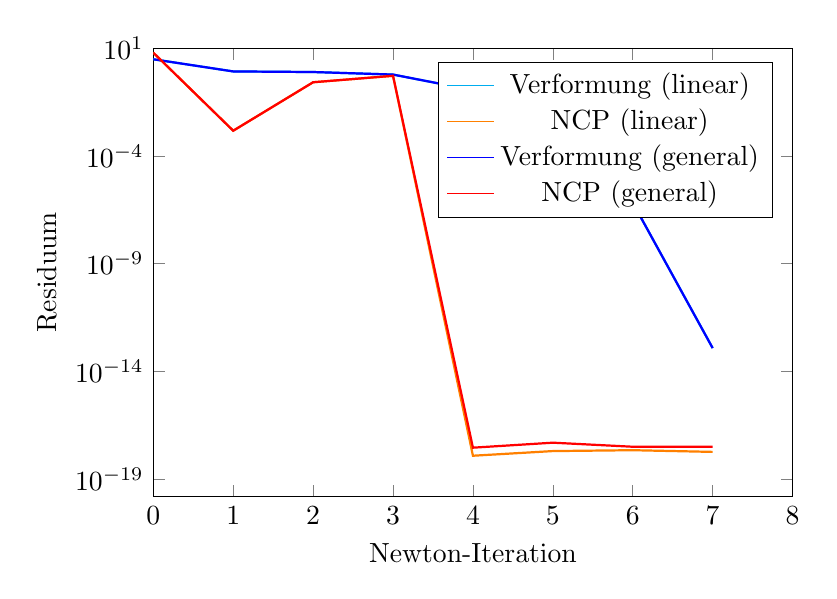
\begin{tikzpicture}[every plot/.append style={thick}] 
\begin{axis}[ 
label style={font=\normalsize}, 
xlabel={Newton-Iteration}, 
ylabel={Residuum}, 
xmin=0, xmax=8, 
ymode=log, 
ymin=0, ymax=10, 
width=0.8\textwidth, 
height=0.6\textwidth, 
legend pos=north east, 
legend style={cells={align=left}}, 
grid style=dashed, 
] 
\addplot[ 
color=cyan, 
] 
coordinates { 
(0, 3.05e+00)(1, 8.33e-01)(2, 7.82e-01)(3, 5.96e-01)(4, 1.13e-01)(5, 1.74e-03)(6, 6.79e-07)(7, 1.23e-13)}; 
\addlegendentry{Verformung (linear)} 
\addplot[ 
color=orange, 
] 
coordinates { 
(0, 6.17e+00)(1, 1.48e-03)(2, 2.62e-01)(3, 5.22e-01)(4, 1.24e-18)(5, 2.04e-18)(6, 2.24e-18)(7, 1.87e-18)}; 
\addlegendentry{NCP (linear)} 
\addplot[ 
color=blue, 
] 
coordinates { 
(0, 3.05e+00)(1, 8.33e-01)(2, 7.82e-01)(3, 5.96e-01)(4, 1.13e-01)(5, 1.74e-03)(6, 6.79e-07)(7, 1.22e-13)}; 
\addlegendentry{Verformung (general)} 
\addplot[ 
color=red, 
] 
coordinates { 
(0, 6.17e+00)(1, 1.48e-03)(2, 2.62e-01)(3, 5.22e-01)(4, 2.93e-18)(5, 5.00e-18)(6, 3.24e-18)(7, 3.24e-18)}; 
\addlegendentry{NCP (general)} 
\end{axis} 
\end{tikzpicture} 
\caption{Residuen des Stoffgesetzes 'Neo Hooke' mit Hinderniss 'Spitze' und 2178 Freiheitsgraden für die Verschiebung.} 
\label{fiq:NeoHooke_Spitze_level4} 
\end{figure} 
